\documentclass[a4paper, 14pt]{extarticle}
\usepackage[left=2cm,right=2cm,top=2cm,bottom=2cm,bindingoffset=0cm]{geometry}
\usepackage[utf8]{inputenc}
\usepackage[english, russian]{babel}
\usepackage{amssymb, latexsym, amsmath}
\usepackage{indentfirst}
\usepackage{graphicx}
\usepackage{citehack}
\usepackage{tabularx}
\usepackage{listings}
\usepackage{pdfpages}

\lstloadlanguages{HTML,python}
\lstset{extendedchars=false,
  breaklines=true,
  breakatwhitespace=true,
  keepspaces = true,
  tabsize=2
}


\begin{document}
\begin{titlepage}

\newpage

\begin{center}
Московский Авиационный Институт \\*
(национальный исследовательский университет) \\*

\vspace{2em}

Факультет прикладной математики и физики \\*
Кафедра вычислительной математики и программирования

\vspace{10em}

\Large \textbf{Курсовой проект \\*
по дисциплине <<Информационные технологии в проектировании и производстве>>} \\*

\vspace{3em}

<<Разработка проектного офиса <<Цифромед>>
\end{center}

\vspace{8em}

\hspace{25em}\vbox{
  \hbox{\bfseries{Выполнил:}}
  \hbox{\hspace{1em} Данилычев И.\,А.}
}

\vspace{2em}

\hspace{25em}\vbox{
  \hbox{\bfseries{Руководитель:}}
  \hbox{\hspace{1em} Скородумов С.\,В.}
}

\vspace{\fill}

\begin{center}
Москва, 2015
\end{center}

\end{titlepage}

\newpage


\tableofcontents
\newpage


\section{Введение}
Планирование -- один из ключевых видов деятельности, необходимых для успешного менеджмента и реализации любого проекта, когда речь заходит о бизнесе. Целью данной работы являлось создание веб-сервиса, оформленного в виде SaaS-решения и представляющего собой проектный офис для совместной работы проектных команд.

В работе представлен процесс проектирования архитектуры и анализа бизнес-логики реализуемого приложения; кроме того, приведено краткое описание проектирования интерфейса (клиентской части). Всё это входило в мою часть работы, определённую через Work Breakdown Structure при планировании проекта.


\begin{figure}[!htb]
  \centering
    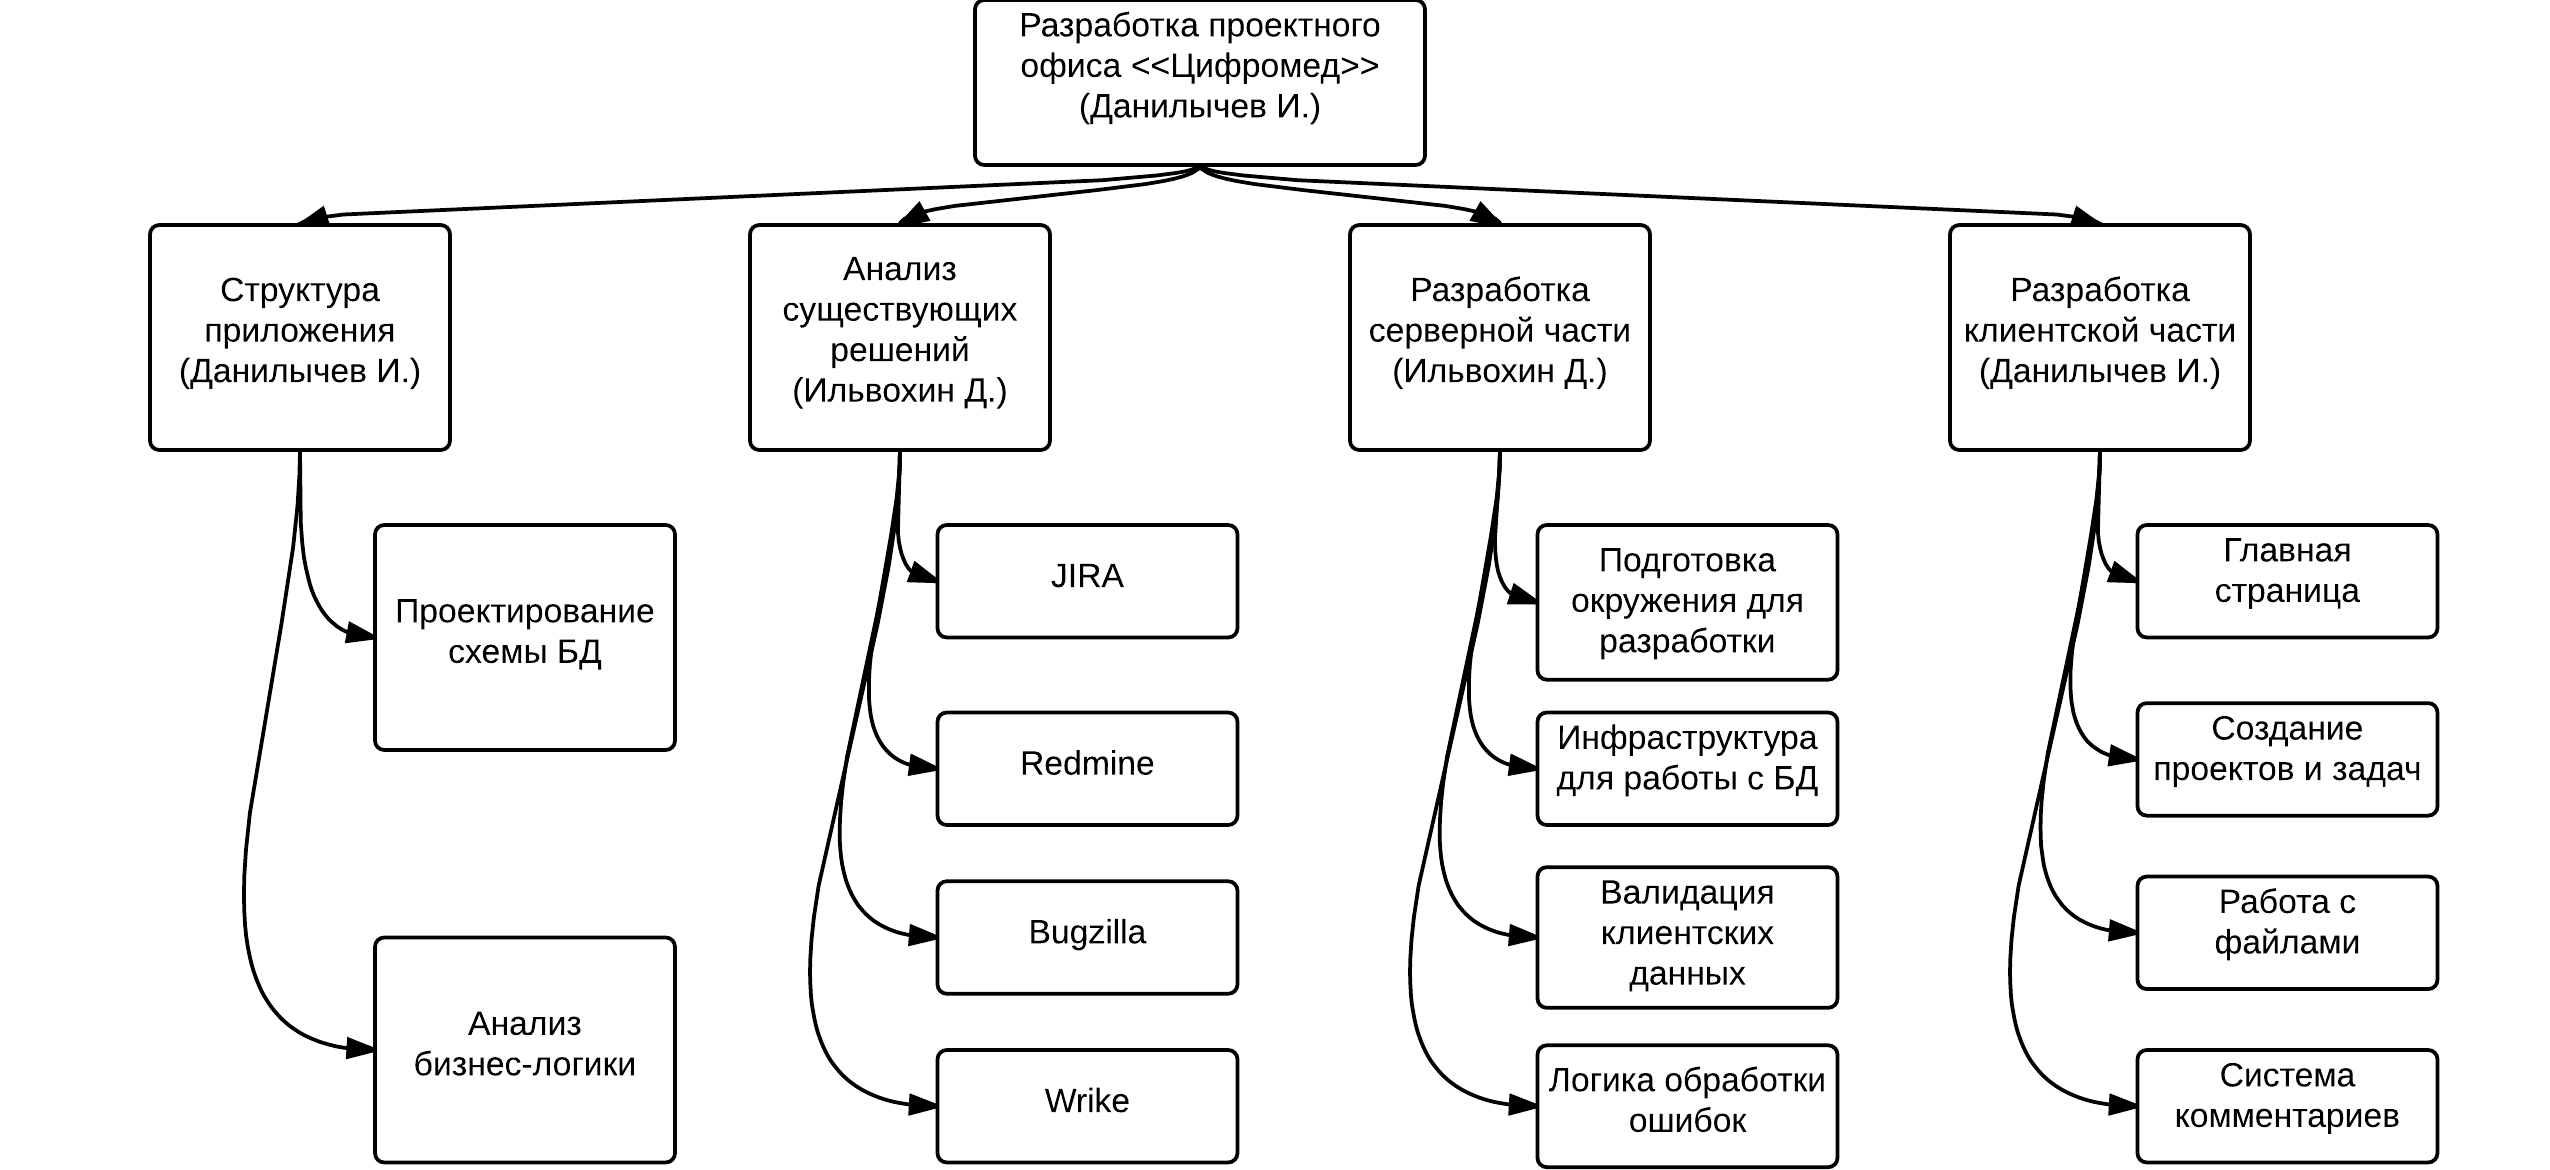
\includegraphics[scale=0.25]{../shared_images/wbs.png}
   \caption{WBS}
    \label{fig:start}
\end{figure}

\newpage

\section{Проектирование приложения}
\subsection{Схема БД}

\begin{figure}[!htb]
  \centering
    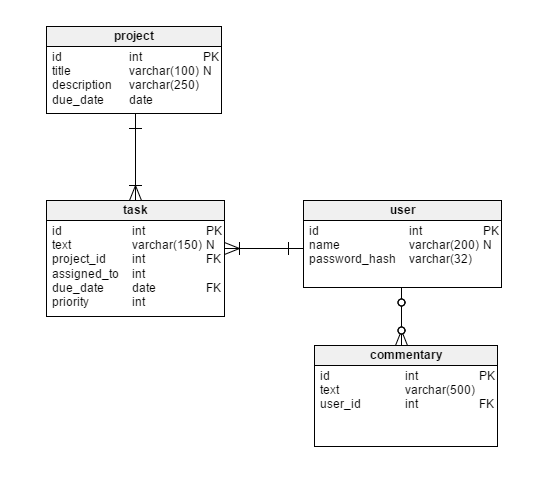
\includegraphics[scale=0.6]{../shared_images/schema.png}
   \caption{Схема БД}
    \label{fig:start}
\end{figure}

Как видно из схемы, ключевой сущностью является проект, который может иметь в своём составе одну или более задач. Задача, в свою очередь, связана с конкретным пользователем, ответственным за её сдачу, с помощью поля {\tt assigned\_to}.

У пользователей имеется возможность оставлять комментарии к задачам, используя реализованную на сайте систему комментариев. Каждый пользователь может как оставлять комментарии, так и не иметь их вообще.

Несмотря на произошедший позднее отказ от реляционных баз данных и переход к БД, основанных на технологии NoSQL, когда вся база представлена коллекцией документов различных типов без разбиения их на таблицы, спроектированная схема легла в основу финальной версии приложения.

\subsection{Анализ места размещения бизнес-логики}
\begin{figure}[!htb]
  \centering
    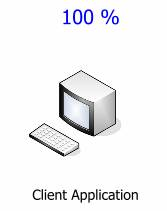
\includegraphics[scale=0.6]{../shared_images/business-logic/client.jpg}
   \caption{Клиентское приложение}
    \label{fig:start}
\end{figure}

На настольных приложениях бизнес-логика содержится на одном звене со всеми остальными слоями. Поскольку нет необходимости разделять слои, они зачастую перемешаны и не имеют четких границ.

\begin{figure}[!htb]
  \centering
    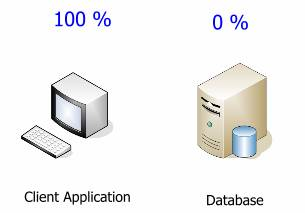
\includegraphics[scale=0.6]{../shared_images/business-logic/client-server.jpg}
   \caption{Приложение с архитектурой «клиент-сервер»}
    \label{fig:start}
\end{figure}


В клиент-серверном приложении имеются два звена, что приводит к созданию как минимум двух слоев. На начальном этапе сервер рассматривается только как удаленная база данных, и деление совпадает с рисунком -- приложение на клиенте и данные на сервере. Обычно вся бизнес-логика находится на клиенте, перемешанная с остальными слоями, такими как пользовательский интерфейс.

Достаточно быстро стало понятно, что можно сократить нагрузку на сеть и централизовать логику для уменьшения постоянных затрат на развертывание, перенеся большую часть бизнес-логики на сервер. Архитектурно сервер является хорошо подготовленным местом в клиент-серверной системе, хотя база данных как платформа даёт мало возможностей. БД были спроектированы для хранения и выдачи и в их архитектуру не были заложены возможности расширения в направлении бизнес-логики. Языки хранимых процедур в базах данных были разработаны для базовых преобразований данных, чтобы поддержать то, на что не хватало SQL. Языки хранимых процедур разработали для быстрого исполнения, а не для обслуживания сложных задач бизнес-логики.

Тем не менее, во избежание переусложнённости клиента часть бизнес-логики была перемещена в хранимые процедуры.

\begin{figure}[!htb]
  \centering
    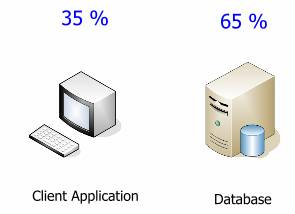
\includegraphics[scale=0.6]{../shared_images/business-logic/client-server-2.jpg}
   \caption{Часть логики хранится на сервере}
    \label{fig:start}
\end{figure}


Когда проблема клиент-серверной архитектуры стала явной, возросла популярность 3-х звенного подхода. Наибольшей и самой тяжелой проблемой того времени было количество подключений. Сейчас многие базы данных могут обрабатывать тысячи единовременных подключений, однако десятилетие или два назад большинство баз данных падало где-то на пятиста подключениях.

Стало популярным объединение подключений в пул, однако для реализации пула подключений в системе с множеством отдельных клиентов, необходимо внедрить третье звено между клиентом и сервером. Среднее звено так и стало называться «среднее звено». В большинстве случаев среднее звено существовало только для управления пулом соединений, но в некоторых случаях бизнес-логика начала перемещаться в среднее звено потому, что языки разработки (C++, VB, Delphi, Java) гораздо лучше подходили для реализации бизнес-логики, чем языки хранимых процедур. Вскоре стало очевидно, что среднее звено -- это наилучшее место для бизнес-логики, и схема приложения трансформировалась:

\begin{figure}[!htb]
  \centering
    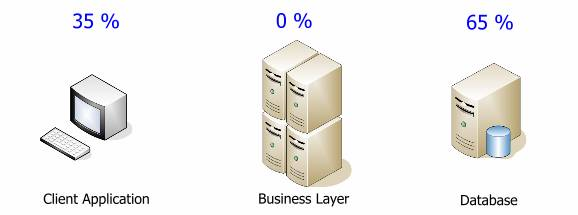
\includegraphics[scale=0.6]{../shared_images/business-logic/client-server-business.jpg}
   \caption{Пустой слой бизнес-логики}
    \label{fig:start}
\end{figure}

В таких случаях бизнес-слой не содержит бизнес правил. Это не настоящий бизнес-слой, а только форматтер XML (или другого потокового формата) и адаптер наборов данных базы данных. Хотя некоторые плюсы, такие как пул соединений и изоляция БД, могут быть достигнуты, это не настоящий слой бизнес-логики, скорее, инородный физический слой без слоя логики.

\begin{figure}[!htb]
  \centering
    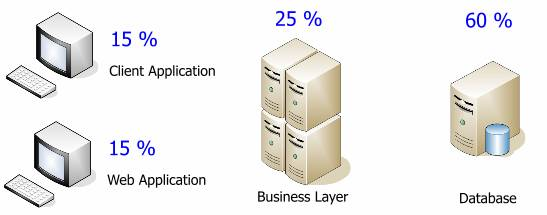
\includegraphics[scale=0.6]{../shared_images/business-logic/client-server-business-2.jpg}
   \caption{Слой бизнес-логики, частично разгружающий БД}
    \label{fig:start}
\end{figure}

Обычно некоторые бизнес-правила приложения переходят в бизнес-слой, но то, что было в базе данных, так в ней большей частью и остается. При повторном использовании бизнес-слоя в таких разработках бизнес-правила должны повторяться и в клиентском приложении. Это сводит на нет основную цель внедрения бизнес-слоя.

\begin{figure}[!htb]
  \centering
    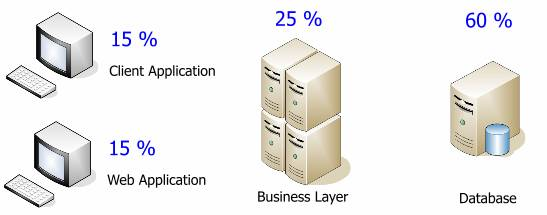
\includegraphics[scale=0.6]{../shared_images/business-logic/client-server-business-2.jpg}
   \caption{Полностью заполненный слой бизнес-логики}
    \label{fig:start}
\end{figure}

Тем не менее, идеальной моделью в данном случае является консолидированная модель, приведённая выше, когда вся бизнес-логика выделена из БД. Такая разработка имеет следующие преимущества:

\begin{itemize}
  \item Вся бизнес-логика находится в одном месте и может быть легко проверена, отлажена и изменена.
  \item Для реализации бизнес правил может быть использован нормальный язык разработки. В нашем случае таким языком стал Python, который больше подходит для данной задачи, чем SQL и хранимые процедуры.
  \item База данных становится слоем хранения и может заниматься эффективным получением и хранением данных без ограничений относящихся к слою бизнес-логики или представления.
\end{itemize}

Кроме того, основным преимуществом становится полное отделение от БД: вся работа с БД ведётся через адаптер, без привязки к конкретной технологии, будь то стэк Oracle или PostgreSQL. При необходимости могут быть составлены механизмы миграции, но бизнес-логика останется в неизменном виде. Как уже было сказано, это снимает лишнюю нагрузку с БД, что, в свою очередь, открывает широкие просторы для масштабирования:

\begin{figure}[!htb]
  \centering
    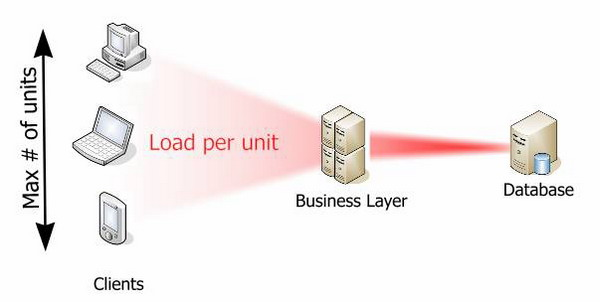
\includegraphics[scale=0.5]{../shared_images/business-logic/scaling.jpg}
   \caption{Поток данных и нагрузка}
    \label{fig:start}
\end{figure}

Перемещая вычисления в среднее звено, команда разработчиков отходит от границ слоя данных, что является несомненным плюсом: в то время как бизнес-звено имеет возможности масштабирования (можно закупить дополнительные сервера для обработки данных), попытка аналогичным образом увеличить количество серверов для хранения данных выльется в проблемы с дублированием, резервным копированием и -- возможно -- миграцией данных, что повлечёт замедление свежерасширенного слоя БД.

\section{Проектирование клиентской части}
\subsection{Главная страница}
Первоначально на главной странице предполагалось выводить последние 10 созданных проектов, чтобы <<прорекламировать>> их остальным участникам и информационно насытить страницу, но поздней было принято решение не показывать ничего, кроме приглашения к логину. Сделано это было по причине того, что список проектов -- без возможности просмотра их незарегистрированным пользователем -- сам по себе не имеет никакого смысла; в результате при просмотре главной страницы незалогиненному пользователю предлагается залогиниться или зарегистрироваться.

\begin{figure}[!htb]
  \centering
    
\includegraphics[scale=0.75]{../shared_images/frontend/title-not-logged-in.png}
   \caption{Титульная страница глазами незарегистрированного пользователя}
    \label{fig:start}
\end{figure}

После логина вниманию пользователя предлагается три списка:

\begin{enumerate}
\item Список задач, в которых пользователь участвует (ответственен за их сдачу). Задачи отсортированы по крайнему сроку (deadline) и имеют, в зависимости от приоритета, различную окраску.
\item Список задач, созданных пользователем. Предназначен для менеджеров, следящих за активностью подчинённых.
\item Список проектов, созданных пользователем. Имеет то же значение, позволяя быстро просматривать задачи отдельного проекта и оценивать объём работы.
\end{enumerate}

\begin{figure}[!htb]
  \centering
    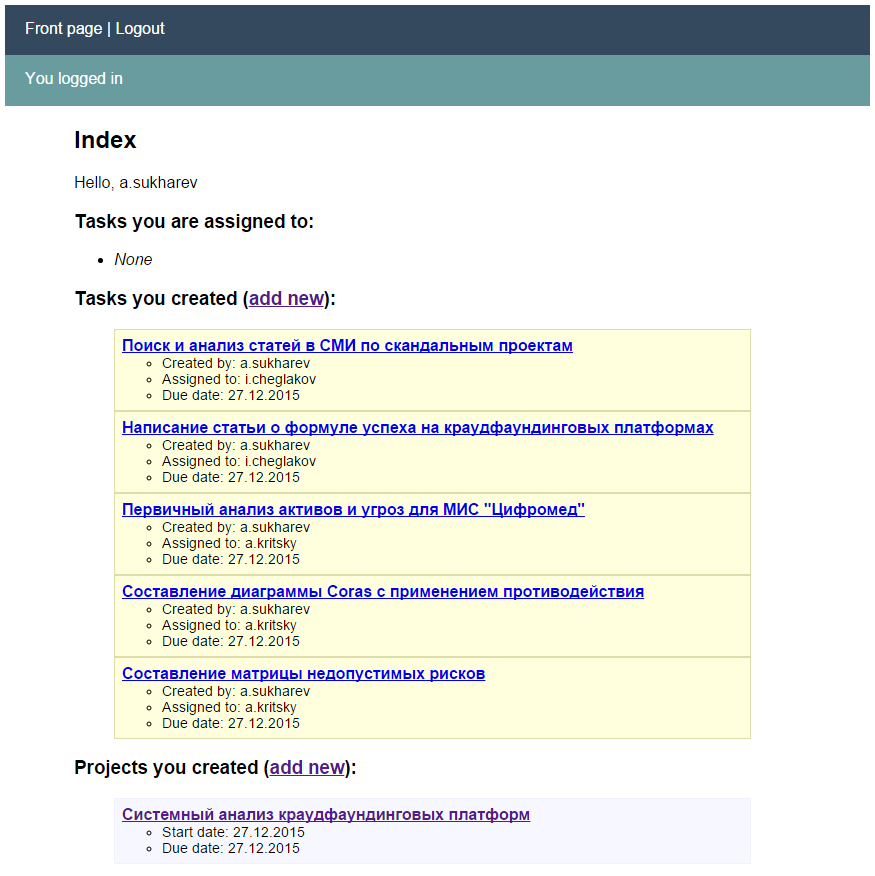
\includegraphics[scale=0.8]{../shared_images/frontend/title-logged-in.png}
   \caption{Титульная страница для участника или PM}
    \label{fig:start}
\end{figure}

\subsection{Создание проектов и задач}
Было решено воспользоваться успешно зарекомендовавшим себя интерфейсом вида <<Заголовок -- поле для заполнения>>. Отдельно стоит упомянуть, что через процедуру создания или редактирования к задаче можно добавить до трёх файлов, связанных с ней.

\begin{figure}[!htb]
  \centering
    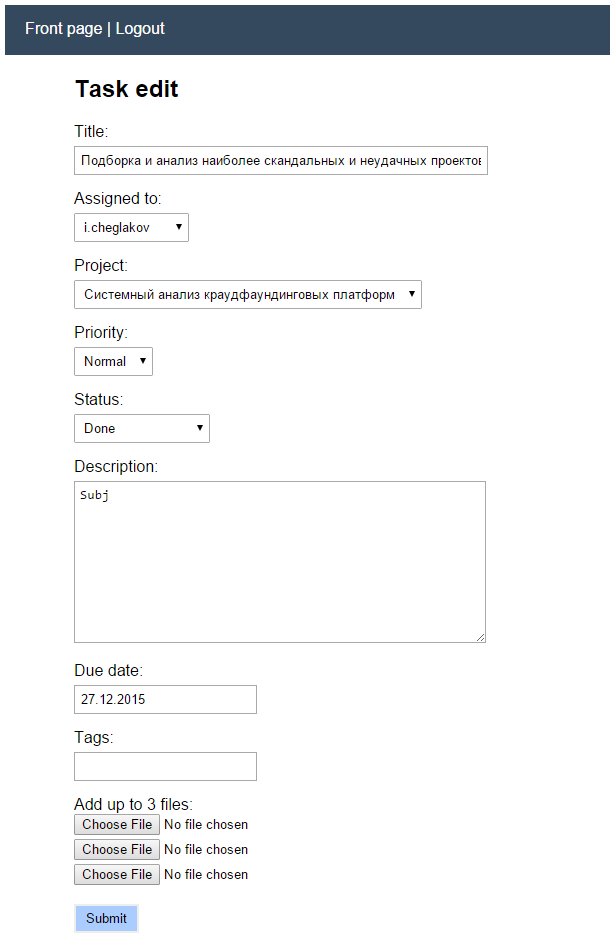
\includegraphics[scale=0.6]{../shared_images/frontend/task-edit.png}
   \caption{Форма редактирования задачи}
    \label{fig:start}
\end{figure}

\begin{figure}[!htb]
  \centering
    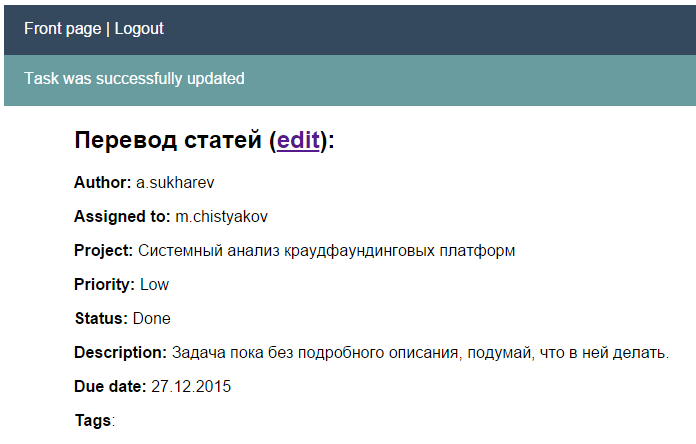
\includegraphics[scale=0.6]{../shared_images/frontend/task-view.png}
   \caption{Страница задачи}
    \label{fig:start}
\end{figure}

\subsection{Работа с файлами}

После информации о каждой задаче выводится список файлов, связанных с ней. По умолчанию файлы сохраняются по пути {\tt /uploads/TASK\_ID/FILENAME} и могут быть просмотрены любым человеком, имеющим ссылку. Тем не менее, ввиду сложности подбора ID (идентификационного номера) задачи, доступ извне к файлам затруднён. Данный принцип обеспечения безопасности называется security through obscurity, или <<безопасность через неясность>>. Его основная идея заключается в том, чтобы скрыть внутреннее устройство системы или реализацию для обеспечения безопасности.

\begin{figure}[!htb]
  \centering
    
\includegraphics[scale=0.75]{../shared_images/frontend/files.png}
   \caption{Список прикреплённых файлов}
    \label{fig:start}
\end{figure}

Стоит отметить, что неосторожный пользователь или злоумышленник не сможет затереть ранее залитый файл, поскольку при конфликте имён к имени нового файла добавляется случайный набор из 8 цифр и латинских букв. Типичная ссылка на файл в результате выглядит так: \\
{\tt http://127.0.0.1:1337/uploads/df0c17989df6268ec08cbc07e9962406/ \\
course-a1a70673.rar}

\subsection{Система комментариев}

Внизу каждой задачи имеется поле для оставления комментариев, а над ним -- список комментариев, отсортированный под дате добавления. Данная система позволяет осуществлять ведение дискуссий по теме задачи.

\begin{figure}[!htb]
  \centering
    
\includegraphics[scale=0.6]{../shared_images/frontend/comments.png}
   \caption{Комментарии к задаче}
    \label{fig:start}
\end{figure}

\section{Заключение}
В рамках проделанной работы была спроектирована схема базы данных, лёгшая впоследствии в основу архитектуры проекта. После детального анализа оптимального места размещения бизнес-логики для неё был выделен отдельный слой, что повлекло за собой отвязку проекта от реляционных БД и конкретных решений в принципе, добавляя приложению гибкости.

Также был спроектирован интерфейс приложения, состоящий из четырёх основных (не считая тривиальных) компонент, обеспечивающий удобную навигацию и ориентировку в списке имеющихся задач и их приоритетов.

\addcontentsline{toc}{section}{Список использованных источников}
\begin{thebibliography}{}
\bibitem{} Википедия [Электронный ресурс]: \\https://ru.wikipedia.org/wiki/Бизнес-логика
\bibitem{} Chad Z. Hower ``Dude, where's my business logic?'' [Электронный ресурс]: http://www.codeproject.com/Articles/10746/Dude-where-s-my-business-logic
\bibitem{} Руководство по проектированию реляционных баз данных [Электронный ресурс]: http://habrahabr.ru/post/193136/
\bibitem{} Глеб Арестов <<Три правила проектирования интерфейсов>> [Электронный ресурс]: http://habrahabr.ru/post/211659/
\end{thebibliography}

\end{document}
